% Ch.8 Robustness (~8-10 pp, dedicated). Analysis Day 8, write-up Day 9.
\chapter{Robustness}
\label{ch:robustness}

\section{Out-of-Sample Predictability}
\label{sec:rob-oos}
% Fully-recursive factors and Campbell-Thompson OOS R^2 (oos.R; plots.R s8_*).
\begin{figure}[t]\centering
  
\includegraphics[width=0.9\linewidth]{figures/s8_r2_oos_pooled.pdf}
  \caption{Out-of-sample $R^2$ (pooled), recursive factors vs recursive mean.}
  \label{fig:s8-oos}
\end{figure}

\section{Subsample Stability}
\label{sec:rob-subsample}
% Pre-/post-2007 (or alternative break); do the headline results hold?

\section{Alternative Global-Factor Construction}
\label{sec:rob-weights}
% Alternative GDP weights; top-down vs bottom-up FXGCF; leave-own-out (FXGCF_lou,
% plots.R s7_*) to remove own-inclusion bias.
\begin{figure}[t]\centering
  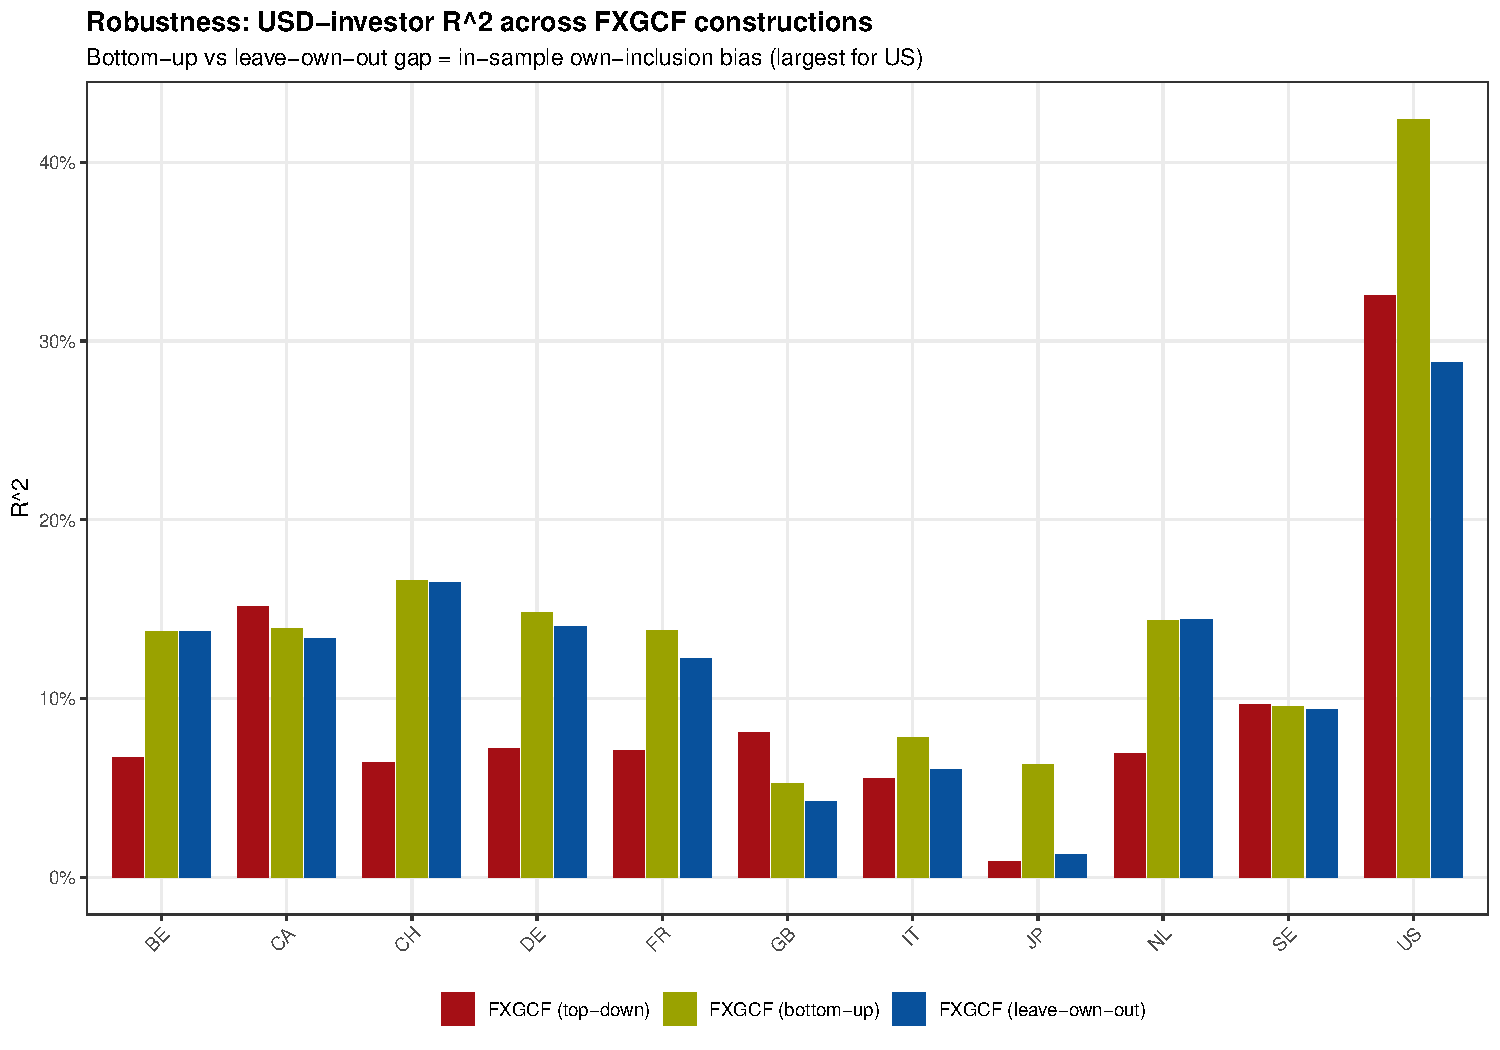
\includegraphics[width=0.9\linewidth]{figures/s7_rob_fxgcf_r2.pdf}
  \caption{FXGCF robustness: top-down vs bottom-up and leave-own-out.}
  \label{fig:s7-rob}
\end{figure}

\section{Cycle Factor versus the Cochrane--Piazzesi Factor}
\label{sec:rob-cf-cp}
% Head-to-head CF vs CP / GCF vs GCP, in-sample and OOS (plots.R s10_*).
\begin{figure}[t]\centering
  
\includegraphics[width=0.9\linewidth]{figures/s10_r2_oos_compare.pdf}
  \caption{Cycle vs forward-based factors: out-of-sample $R^2$.}
  \label{fig:s10-cmp}
\end{figure}

\section{Sensitivity to Construction Choices}
\label{sec:rob-sensitivity}
% EWMA decay v, window M, and the maturity menu. State which results are
% fragile and which survive.
